% !TeX spellcheck = de_CH
\documentclass[
a4paper,
oneside,
10pt,
fleqn,
headsepline,
toc=listofnumbered, 
bibliography=totocnumbered]{scrartcl}

% deutsche Trennmuster etc.
\usepackage[T1]{fontenc}
\usepackage[utf8]{inputenc}
\usepackage[english, ngerman]{babel} % \selectlanguage{english} if  needed
\usepackage{lmodern} % use modern latin fonts

% Custom commands
\newcommand{\AUTHOR}{M. Wieland}
\newcommand{\SECONDAUTHOR}{F. Hauser}
\newcommand{\THIRDAUTHOR}{M. Trentini}
\newcommand{\FOURTHAUTHOR}{P. Scherler}
\newcommand{\INSTITUTE}{Hochschule für Technik Rapperswil}
\newcommand{\LECTURER}{Prof. Dr. Jürg Stadelwieser}
\newcommand{\GITHUB}{https://github.com/michiwieland/businessplan}

% Jede Überschrift 1 auf neuer Seite
\let\stdsection\section
\renewcommand\section{\clearpage\stdsection}

\makeatletter
\newcommand\invisiblesection[1]{%
	\refstepcounter{section}%
	\addcontentsline{toc}{section}{\protect\numberline{\thesection}#1}%
	\sectionmark{#1}\phantom{}}
\makeatother

% Multiple Authors
\usepackage{authblk}

% Include external pdf
\usepackage{pdfpages}

% Layout / Seitenränder
\usepackage{geometry}

% Inhaltsverzeichnis
\usepackage{makeidx} 
\makeindex

\usepackage{url}
\usepackage[pdfborder={0 0 0}]{hyperref}
\usepackage[all]{hypcap}
\usepackage{hyperxmp} % for license metadata

% Glossar und Abkürzungsverzeichnis
\usepackage[acronym,toc,nopostdot]{glossaries}
\glossarystyle{altlisthypergroup}
\usepackage{xparse}
\DeclareDocumentCommand{\newdualentry}{ O{} O{} m m m m } {
	\newglossaryentry{gls-#3}{name={#5},text={#5\glsadd{#3}},
		description={#6},#1
	}
	\makeglossaries
	\newacronym[see={[Siehe:]{gls-#3}},#2]{#3}{#4}{#5\glsadd{gls-#3}}
}
\makeglossaries

% Mathematik
\usepackage{amsmath}
\usepackage{amssymb}
\usepackage{amsfonts}
\usepackage{enumitem}

% Images
\usepackage{graphicx}
\graphicspath{{images/}} % default paths

%figures
\usepackage{tikz}
\usetikzlibrary{shapes.geometric}

%risk-rating
\newcommand\risk[2]{
	\begin{tikzpicture}
	\draw [thick, |->] (0,2) -- (#2,2);
	\draw [fill=red, thick] (#1,2) circle [radius=0.2];
	\end{tikzpicture}
}

% Boxes
\usepackage{fancybox}

%Tables
\usepackage{tabu}
\usepackage{booktabs} % toprule, midrule, bottomrule
\usepackage{array} % for matrix tables

% Multi Columns
\usepackage{multicol}

% Header and footer
\usepackage{scrlayer-scrpage}
\setkomafont{pagehead}{\normalfont}
\setkomafont{pagefoot}{\normalfont}
\automark*{section}
\clearpairofpagestyles
\ihead{\headmark}
\ohead{\TITLE}
\cfoot{\pagemark}

% Pseudocode
\usepackage{algorithm}
\usepackage{algorithmic}

% Code Listings
\usepackage{listings}
\usepackage{color}
\usepackage{beramono}

\definecolor{DarkPurple}{rgb}{0.4, 0.1, 0.4}
\definecolor{DarkCyan}{rgb}{0.0, 0.5, 0.4}
\definecolor{LightLime}{rgb}{0.3, 0.5, 0.4}
\definecolor{Blue}{rgb}{0.0, 0.0, 1.0}

\lstdefinestyle{eclipse-style}{
	language=Java,
	columns=flexible,
	showstringspaces=false,
	basicstyle=\footnotesize\ttfamily, 
	keywordstyle=\bfseries\color{DarkPurple},
	commentstyle=\color{LightLime},
	stringstyle=\color{Blue}, 
	escapeinside={£}{£}, % latex scope within code
	morekeywords={length},
	numbers=left,
	numberstyle=\tiny\color{black},
	frame=single,
}
\lstset{style=eclipse-style}


% Theorems \begin{mytheo}{title}{label}
\usepackage{tcolorbox}
\tcbuselibrary{theorems}
\newtcbtheorem[number within=section]{definiton}{Definition}%
{fonttitle=\bfseries}{def}
\newtcbtheorem[number within=section]{remember}{Merke}%
{fonttitle=\bfseries}{rem}
\newtcbtheorem[number within=section]{hint}{Hinweis}%
{fonttitle=\bfseries}{hnt}

% Dokumentinformationen
\newcommand{\SUBJECT}{Businessplan}
\newcommand{\TITLE}{GitFit}

\pagenumbering{Alph}
% pdf metadata
\hypersetup{
	pdfauthor={\AUTHOR},
	pdftitle={\SUBJECT \TITLE}
}

\begin{document}


% German \and
\renewcommand\Authands{ und }
% Front page
\title{\TITLE}
\subject{\SUBJECT}
\author{\SECONDAUTHOR}
\author{\THIRDAUTHOR}
\author{\FOURTHAUTHOR}
\author{\AUTHOR}
\affil{\INSTITUTE}
\affil{\LECTURER}
\date{\today}
\maketitle

\pagecolor{PrimaryColor}\afterpage{\nopagecolor}

\begin{center}
	
\includegraphics[width=0.7\linewidth]{images/front}
\end{center}


\color{black}


% Table of contents
\tableofcontents


% Glossar and acronyms (if included \loadglsentries{glossar})
\printglossary[type=\acronymtype]
\printglossary
\glsaddall


%TODO Total: 20 Seiten -> Es muss ersichtlich sein, was das Produkt bringt.
%TODO Sturktur nach PWC -> Siehe PDF auf Skripte Server

% TODO: Hoher Preis in K.6 wiederspruch zu tiefer Preis in K.2

\clearpage

\section{Management Summary}

\pagestyle{headings}
\pagenumbering{arabic}

Schweizer Fitnesscenter arbeiten heute vorzugsweise mit Stift und Papier, um die Trainingspläne ihrer Kunden zu verwalten. Dies hat einen entscheidenden Nachteil: Die Auswertung ist stark limitiert.

\hfill \\
GitFit ist eine umfassende Lösung für Fitnesscenter, um ihren Kunden ein neuartiges Trainingserlebnis zu bieten. Die Dienstleistung besteht aus einer benutzerfreundlichen App, sowie einer Plattform, über welche sich die teilnehmenden Fitnesscenter austauschen können. Die gesamte Infrastruktur wird von GitFit betrieben. GitFit erlaubt es effiziente und praxisorientierte Trainingspläne zu erstellen und diese komfortable auszuwerten.  
\hfill \\ \\
Die Schweizer Fitnessbranche floriert, gerade durch anhaltenden Trend von einem gesunden und ausgeglichenen Lifestyle. GitFit setzt hier an und liefert ein Produkt, von dem in erster Linie die Fitnesscenter, im Endeffekt aber auch der Endkunde (im weiteren der Sportler genannt) profitiert.  

\hfill \\
Falls die für den Finanzplan getroffenen Annahmen eintreffen, erwarten wir im ersten Geschäftsjahr einen Gewinn von [??]. Dieser wird sich [??] verhalten.


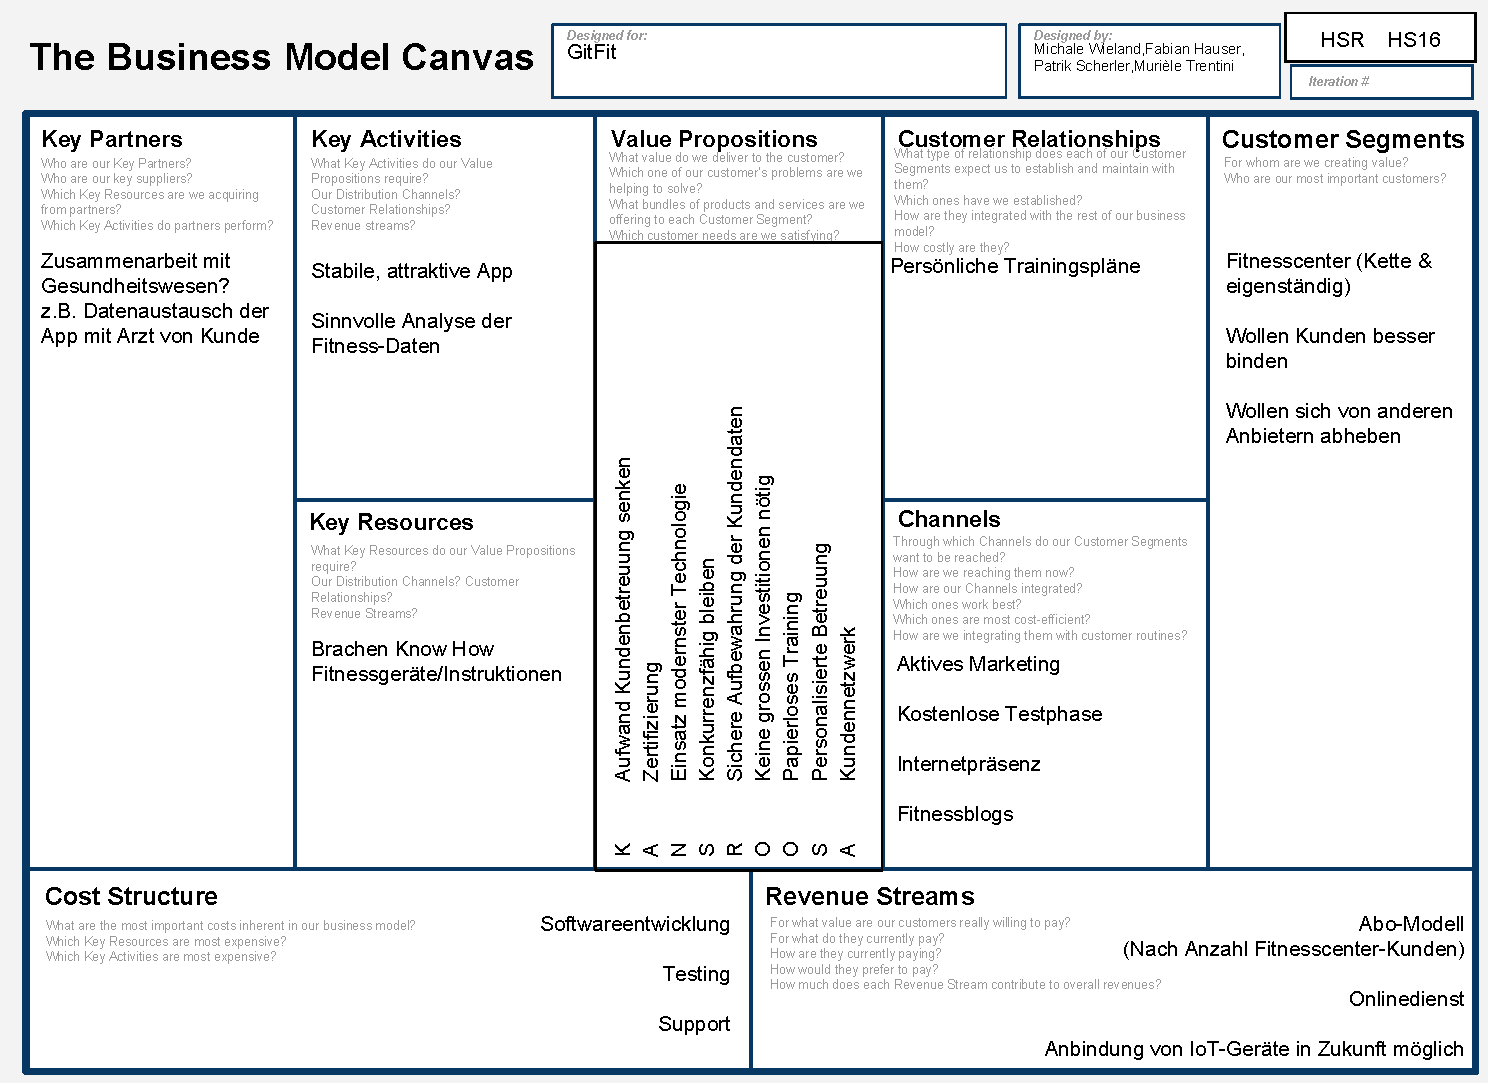
\includepdf[pages=-,addtotoc={1, section, 1, Business Model Canvas, p1},landscape=true]{images/businessmodelcanvas.pdf}
%TODO: Fix title and pdf --> on one page!

\clearpage
\section{Mission, Vision und Strategie: die Zukunft}
\subsection{Mission}
Unsere Aufgabe ist es, vielen Menschen ein völlig neues Erlebnis für ein persönliches Training im Fitnesscenter zu bieten. Wir tun dies, indem wir eine App anbieten, welche die Fitnesslandschaft revolutioniert. Dies mit einem bisher unerreichtem Mass an Komfort.

\subsection{Vision}
Schweizer Fitnesscenter setzen aktuell vorzugsweise auf Papier und Bleistift für die Trainingsplanung ihrer Kunden. Dies ist nicht mehr zeitgemäss und bedarf einer Generalüberholung. Am Puls der Zeit zu sein, bedeutet für ein Fitnesscenter einen modernen und attraktiven Dienstleister für seine Kunden darzustellen. Die Digitalisierung bietet unendlich viele Möglichkeiten, die es zu nutzen gilt. \\
Wir wollen eine App kreieren, welche die Fitnessbranche wieder auf den aktuellen Stand der Technik katapultiert. Die App bietet aufschlussreiche Statistiken sowie hilfreiche Tipps zu Übungen, wenn der Trainer gerade nicht in der Nähe ist.

\subsection{Strategie}
Unser Angebot richtet sich in erster Linie an grosse Fitnesscenter, da wir glauben, dass diese an einem übergreifenden Wissensaustausch ihrer Filialen interessiert sind. Im Rahmen der Entwicklung kümmern wir uns in einer ersten Phase um das Anreichern von Stammdaten mit auserwählten Partner-Center. Die Daten sollen als solides und realitätsnahes Fundament für die weitere Entwicklung dienen. In einer zweiten Phase wird dann die App für den Endkunden entwickelt, die ein möglichst komfortables und persönliches Trainingserlebnis vermitteln soll. 

\subsubsection{Wettbewerbsstrategie}
Der schweizer Fitnessmarkt boomt und trotzdem ist wenig Digitalisierung in der Branche erkennbar. Ähnliche Projekte finden im Ausland bereits Anklang, jedoch gibt es im Inland keine vergleichbare Dienstleistung. Grund genug, diese Lücke zu füllen. Die Schwierigkeit in dem Projekt liegt deshalb weniger in der Positionierung gegenüber ausländischen Dienstleistern, sondern vielmehr darin, die heimischen Fitnesscenter mit der neuen Technologie vertraut zu machen.


\clearpage
\section{Produkte und Dienstleistungen: die Marktleistung}

\subsection{Die App}
\begin{figure}[h]
\centering
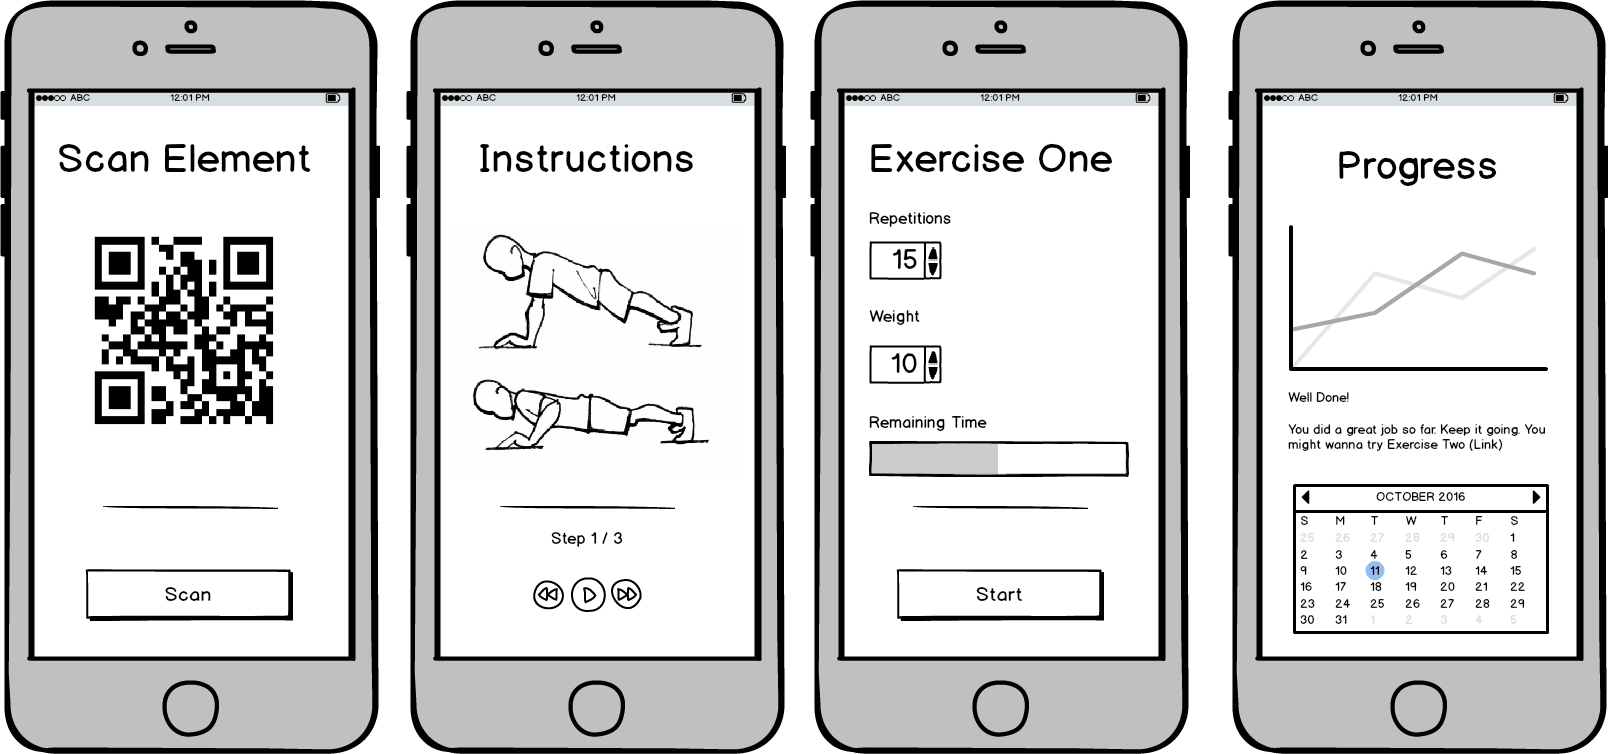
\includegraphics[width=0.5\linewidth]{images/app}
\caption{Wireframe der App}
\label{fig:app}
\end{figure}
Der Kern unseres Angebots bietet die App. In ihr können individuelle Trainingspläne erstellt und Trainingserfolge dokumentiert werden. Übungen können vom Trainer gespeichert und wiederverwendet werden. Dadurch lässt sich auch deren Wirksamkeit auswerten. \\ \\
Durch die Verknüpfung mit Activity-Trackern (z.B. Fitness Armbänder) von Drittanbietern hat der Kunde auch stets den Einfluss des Trainings auf den eigenen Körper im Auge. So kann beispielsweise der Verlauf der Herzschlagfrequenz während einer Übung aufgezeichnet werden. \\ \\
Die ausführliche Analysefunktionen bieten Möglichkeiten zur Planung eines Trainings, dass individuell auf den Kunden zugeschnitten ist und seine aktuelle Leistungsfähigkeit und Gesundheit jederzeit berücksichtigt. Es steigert auch die Motivation des Sportlers, da er seine Fortschritte jederzeit prüfen kann. \\ \\
Der Einsatz unseres Produkts würde ein Fitnesscenter zertifizieren und es so von Mitbewerbern abheben.

\subsection{Dienstleistung}
\begin{figure}[H]
	\centering
	\includegraphics[width=0.5\linewidth]{images/GitFit_concept}
	\caption{Übersicht der verschiedenen Akteure}
	\label{fig:GitFit_concept}
\end{figure}
Nebst der App bietet GitFit ein Gesamtsystem in der Cloud, auf das die Fitnesscenter jederzeit Zugriff haben. Kundendaten werden sicher übertragen und verschlüsselt gespeichert. Dies garantiert ein hohes Mass an Sicherheit und Verfügbarkeit.  \\ \\
Zum einen kann der Betreuer individuelle Trainingspläne für seine Kunden erstellen und hat durch die Analysedaten ein direktes Feedback über deren Trainingserfolge. \\ \\
In Zukunft wäre auch der Einsatz von smarten Fitnessgeräten denkbar, welche sich automatisch (z.B. beim scannen eines QR-Codes) nach dem Trainingsplan des Benutzers einrichten und seine Aktivitäten aufzeichnen.
Zusätzlich könnten so auch Statistiken über die Belegung der Geräte erstellt werden, um Engpässe zu vermeiden. \\ \\
Auch eine Schnittstelle für Hausärzte und Krankenkassen wäre möglich. Beispielsweise um spezialisierte Prämienrabatte anzubieten oder eine bessere Diagnose stellen zu können. \\ \\
Die App ist für den Endkunden gratis. Das Fitnesscenter bezahlt im Abo-Modell, um seine Filiale in der Cloud verfügbar zu machen. Der Preis richtet sich dabei nach der Anzahl Kunden, welche die App nutzen.
\pagebreak
\subsection{Kundennutzen}\label{sec:kundennutzen}
Darstellung des Kundennutzens mit Hilfe des Modells KANSROOSA:
\begin{table}[H]
	\centering
	\begin{tabu} to \linewidth {l l}
		\toprule 
		Bedürfnis & Fitnesscenter \\
		\midrule
		KOMFORT & Aufwand der Kundenbetreuung senken \\
		ANSEHEN & Zertifizierung \\
		NEUHEIT & Einsatz modernster Technologie \\
		SELBSTERHALTUNG & Konkurrenzfähig bleiben \\
		RISIKOLOS & Sichere Aufbewahrung der Kundendaten \\
		ÖKONOMIE & Keine grossen Investitionen nötig \\
		ÖKOLOGIE & Papierloses Training \\
		SYMPATHIE & Personalisierte Betreuung \\
		ANGEHÖRIGKEIT & Kundennetzwerk \\
		\bottomrule 
	\end{tabu} 
	\caption{Anwendung von KANSROOSA an GitFit}
\end{table}


\clearpage
\section{Markt und Kunden: das Zielgebiet}

\subsection{Marktübersicht}

\subsubsection{Marktkapazität / Marktsegmentierung}\label{sec:marktkapazitat}

\paragraph{Fitnesscenter in der Schweiz}
Gemäss einer Studie des BASPO Statistik aus dem Jahre 2014 sind 16\% der Schweizerinnen und Schweizer in einem privaten Fitnesscenter angemeldet \cite{schweizer+fitness}. Damit ist das betreiben eines Fitnesscenters eine lukrative Angelegenheit. In der Schweiz wird die Anzahl auf 700-800 Fitnesscentern im Jahr 2013 geschätzt \cite{fitness-studios+1+milliarde}\cite{fitness+tribune}. \\ \\
Die meisten Fitnesscenter setzten digitale Mittel lediglich zur Verwaltung des Kundenstammes und Administration ein; nach unseren Recherchen sind weitere Verwaltungsapplikationen bisher nicht im Einsatz. \\ \\
Unsere Lösung hat grundsätzlich Marktpotential für alle Betreiber von Fitnesscentern, speziell aber in urbanen Gebieten dürfte das Marktvolumen beträchtlich sein. Wir schätzen, dass wir im Optimalfall längerfristig einen Marktanteil von rund 70\% erreichen können (ca. 30\% der Fitnesscenter bedient Nischenmärkte).

\paragraph{Grössere Fitnesscenter}
In der Schweiz gibt es einige grössere Anbieter, welche mehrere Filialen betreiben. Diese sind interessante Abnehmer für unsere App, da sie viele Kunden und damit entsprechende Datenmengen zu verwalten haben.

Die grössten schweizer Fitnesscenter sind\cite{fitness+tribune}:

\begin{multicols}{2}
	\begin{itemize}
		\item \href{http://mfit.ch/}{MFit}
		\item \href{http://www.activfitness.ch/}{ActiveFitness}
		\item \href{http://fitnessconnection.ch/}{FitnessConnection}
		\item \href{http://www.fitnesspark.ch/}{FitnessPark}
		\item \href{http://holmesplace.ch/de/}{Holmesplace}
		\item \href{http://www.kieser-training.com/}{Kieser Training}
		\item \href{http://www.swiss-training.com/}{Swiss Training}
		\item \href{http://tc-training.ch/}{TC Training}
	\end{itemize}
\end{multicols}

\subsubsection{Marktakteure}
In der Schweiz gibt es bisher keine Anbieter von Apps, welche sich direkt an Fitnesscenter wenden. Wir haben das schweizer App ''myClubs'' angeschaut, das sich direkt an professionelle Sportler oder Amateursportler wendet.
\\ \\
In Deutschland gibt es einige wenige Anbieter von Apps für den Fitnessgebrauch; die meisten richten sich aber an Sportler und gehen nicht auf Fitnesspläne oder interaktion mit Fitnessgeräten ein. Daneben betreiben ein paar Fitnesscenter kleinere Eigenentwicklungen, welche nicht weiter verbreitet sind. Die Firma \emph{eGym} ist ein potentieller direkter Konkurrent.
\\ \\
Mehr Informationen zur potentiellen Konkurrenz sind im Kapitel \ref{sec:konkurrenz-die-mitbewerber} zu finden.


\subsubsection{Erfolgsfaktoren im Markt}

Ein wesentliches Problem von Fitnesscentern ist das halten ihrer Kunden, da inzwischen eine ziemlich ausgebreitete Konkurrenz existiert. Aus diesem Grund werden die Fitnesscenter die App wählen, welche die grösste Kundenbindung ermöglicht. Dabei spielen Design, Qualität und vor allem der gute Ruf eine Rolle. Die Kansroosa-Analyse findet sich im Kapitel \ref{sec:kundennutzen} Kundennutzen.

\subsubsection{Marktentwicklung}
Der Markt für unsere App ist in den letzten Jahren stark gewachsen \cite{fitness-studios+1+milliarde}\cite{fitness+tribune}, allerdings ist es schwierig, genaue Zahlen zu finden. Zunehmend gibt es auch grössere Fitnesscenter (siehe Details im Abschnitt \ref{sec:marktkapazitat}), welche für uns einen interessanten Zielmarkt darstellen.
\\ \\
Aufgrund der beschränkten Zahl an Fitnesscentern ist es wichtig, unsere App gut zu profilieren und relativ schnell einen hohen Bekanntheitsgrad zu erlangen.

\subsection{Chancen und Risiken / Nachfrage \& Charakteristika}

Da in der Schweiz erst wenige Fitnesscenter im digitalen Zeitalter angekommen sind, gibt es hier eine grosse Chance, Fuss auf dem Markt zu fassen. Einmal etabliert ist es für Konkurrenten schwierig, unser Angebot abzulösen.
\\ \\
Das grösste Risiko geht von der deutschen Konkurrenz aus, da diese aufgrund der finanziellen Gegebenheiten das Produkt zu deutlich günstigeren Preisen anbieten können. Mehr Details zur Konkurrenz findet sich im Kapitel \ref{sec:konkurrenz-die-mitbewerber}.


\subsection{Eigene Marktstellung}

Als Startup können wir unsere Firma mit einer neuen Marke etablieren. Bei den Gründungsmitgliedern ist ein gutes technisches Know-How zur App-Entwicklung vorhanden (Informatik B.sc).
\\ \\
Bisher existieren noch keine über die Bedarfsanalyse herausgehende Geschäftskontakte in diesem Bereich.


\subsubsection{Zielmarkt}

Unser Startup konzentriert sich zum Start auf den deutschschweizerischen Markt. Dies aus administrativen und preispolitischen Gründen, damit wir uns auf die deutschsprachige Version und das grösste schweizerische Marktsegment fokussieren können. Zu einem späteren Zeitpunkt ist die Übersetzung und Ausbreitung des Zielmarktes geplant.
\\ \\
Um das Interesse der Fitnesscenter-Betreiber zu gewinnen, wird unser Verkauf nach der Pilotphase direkt mit den Fitnesscentern in Kontakt stehen. Mehr Informationen zum Verkaufs- und Marketingkonzept sind im Kapitel \ref{sec:marketing-der-weg-zum-markt} ersichtlich.


\clearpage
\section{Konkurrenz: die Mitbewerber}\label{sec:konkurrenz-die-mitbewerber}

Auf dem schweizer Markt ist die Konkurrenz noch klein. Erst wenige Fitnesscenter sind im digitalen Zeitalter angekommen. Jedoch gibt es einige Anbieter im nahen Ausland, für welche die Schweiz einen attraktiven Markt bietet. Beide Gruppen wollen wir als potentielle Konkurrenten analysieren.
\subsection{Konkurrenzunternehmen}
\subsubsection{myClubs}
myClubs\cite{myclubs} ist ein schweizer Anbieter einer Fitness App. Ihr Ziel ist es, einem Sportler eine flexible Möglichkeit zu bieten, Sport zu treiben. Dabei legen sie ihren Fokus nicht darauf, Fitnesscenter attraktiver zu gestalten oder zu digitalisieren, sondern dem Sportler ein breites Sportangebot in einem einzigen Abo zu bieten. Im Gegensatz zu unserer Strategie sind die Endkunden von myClub also Sportler, nicht Fitnesscenter.
Das myClubs Angebot umfasst:
\begin{itemize}
	\item Auswahl an verschiedenen Sportarten und -kursen
	\item Auswahl an verschiedenen Partner-Anbietern
	\item Zum Fixpreis im Abosystem (Flatrate)
\end{itemize}
Wir heben uns vom Konkurrenten myClub ab, da wir unseren Fokus auf die Verbesserung des Kraft- und Ausdauertrainings in einem Fitnesscenter legen. Dennoch besteht die Möglichkeit, dass ein Fitnesscenter sich dazu entscheidet, ihr Sportangebot bei myClubs anzubieten und dann davon absieht unsere App zu nutzen.
\paragraph{Risikoeinschätzung} \qquad \risk{4}{5} 4/5
\subsubsection{eGym}
Der deutsche Anbieter eGym\cite{egym} verfolgt sehr ähnliche Ziele wie wir. Sie bieten ihren Partnerfitnesscentern eine App mit folgenden Kernfunktionen:
\begin{itemize}
	\item Zugriff auf den Trainingsplan des Fitnesstrainers
	\item Dokumentation von Trainingseinheiten
	\item Kontrolle über Trainingserfolg und Vergleich mit Kollegen
\end{itemize}
eGym wäre ein starker Konkurrent, falls er in den schweizer Markt expandieren würde.
\paragraph{Risikoeinschätzung} \qquad \risk{3}{5} 3/5
\pagebreak
\subsubsection{Technogym}
Technogym\cite{technogym}ist ein Anbieter aus den Niederlanden. Sie bewegen sich im selben Marktsegment wie wir. Sie verkaufen ihre Fitnessapp sowie angebundene Fitnessgeräte an ihre Fitnesscenter-Kunden.
Ihre Produktpalette umfasst:
\begin{itemize}
	\item Fitnessgeräte mit digitalen Funktionen
	\item vom Trainer erstellte Fitnesspläne mit der Prescribe-App
\end{itemize}
Dabei legen sie ihren Fokus aber vor allem auf den Vertrieb von Fitnessgeräten, wobei wir uns auf die Digitalisierung unserer Kunden konzentrieren.
\paragraph{Risikoeinschätzung} \qquad \risk{2}{5} 2/5
\subsubsection{Freeletics}
Der deutsche Dienstleister Freeletics\cite{freeletics} entwickelt eine eigene Fitness-App und betreibt eine Fitnesscenter-Kette.
Folgendes Angebot bietet Freeletics:
\begin{itemize}
	\item App mit Übungsanleitungen und Fortschrittstracking
	\item Ihre eigene Fitnesscenter-Kette
\end{itemize}
Freeletics wären nur ein ernsthafter Konkurrent, wenn sie in die Schweiz expandieren und hier ansässige Fitnesscenter vom Markt vertreiben würden.
\paragraph{Risikoeinschätzung} \qquad \risk{2}{5} 2/5
\subsection{Konkurrenzanalyse}
\paragraph{Wie arbeitet die Konkurrenz?} \hfill \\
Passend zum Marktsegment haben alle Konkurrenten eine starke Internet-Präsenz mit ansprechenden, modernen Websites. 
Um junge sportbegeisterte Kunden anzusprechen, setzen sie stark auf Social Media Marketing über Facebook, Twitter und Co. Einige betreiben auch einen Blog. Zudem haben sie allgemein eine hohe Medienpräsenz mit Abgabe eines Presse-Kits oder Publi-Reportagen in Zeitschriften. Viele unserer Konkurrenten konzentrieren sich stark auf den Endkunden ''Sportler''.

\begin{figure}[H]
\centering
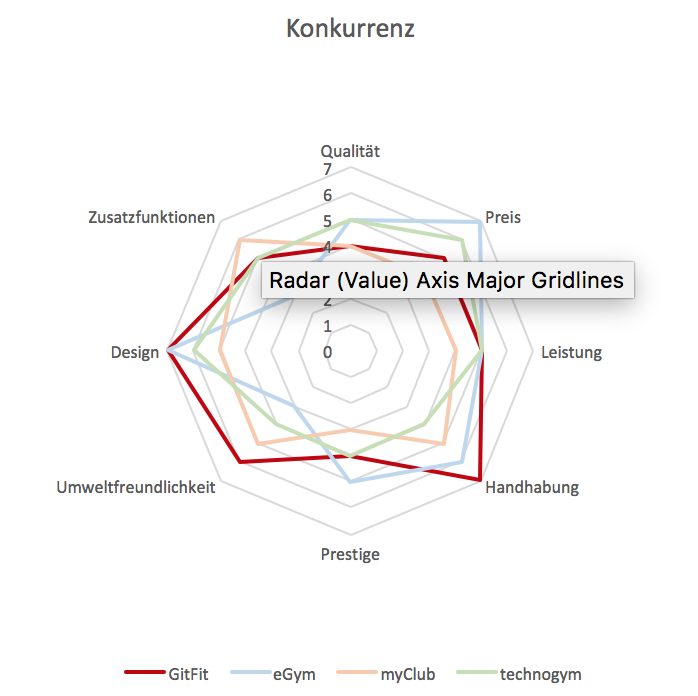
\includegraphics[width=0.9\linewidth]{images/konkurrenz}
\caption{Konkurrenzanalyse}
\label{fig:konkurrenz}
\end{figure}
\paragraph{Konsequenzen}\hfill \\
Aus der Konkurrenzanalyse ergab sich, dass wir uns auf folgende Punkte konzentrieren wollen:
\begin{itemize}
	\item Hoher Preis, dafür sehr gute schweizer Qualität (Label Schweiz)
	\item Modernes Auftreten und Design mit einfacher Handhabung
	\item Wir sprechen direkt Fitnesscenter an, ohne Umweg über den Sportler.
\end{itemize}

\clearpage
\section{Marketing: der Weg zum Markt}\label{sec:marketing-der-weg-zum-markt}

\subsection{Marketingziele}
Um unseren Zielmarkt zu erschliessen, haben wir uns quantitative Ziele gesetzt:
\begin{itemize}
	\item Bis Februar 2017 soll ein Prototyp der App vorgestellt werden können, um neue Kunden von unserer Idee und den damit verbundenen Vorteilen zu überzeugen.
	\item Bis Mai 2017 ist ein starker Partner gefunden, der im Idealfall über mehrere Fitnesscenter in unterschiedlichen deutschschweizer Regionen verfügt.
	\item Bis Ende 2017 ist eine praxisnahe, moderne Trainingsapp entwicket. Die App soll von möglichst vielen Kunden-Inputs profitieren und diese benutzerfreundlich umsetzen.
	\item Bis Sommer 2018 können mindestens 10 weitere Fintnesscenter mit GitFit ausgerüstet werden.
\end{itemize}

\subsection{Marktpositionierung}
Wir setzen primär auf den deutschschweizer Markt, wobei wir uns darauf konzentrieren, eine grosse Fitnesscenter-Kette als Partner zu gewinnen. Da wenige ''Big Player'' die Branche dominieren, wird sich deren Einsatz von GitFit bei den Konkurrenzlinien und kleineren Fitnesscenter herumsprechen. Fitnesscenter die noch auf herkömmliche Arbeitsmethoden setzen, werden als nicht mehr zeitgemäss betrachtet und so zu einer Digitalisierung gezwungen. Wir unterscheiden zwischen zwei Typen von Fitnesscenter, die als Kunden in Frage kommen:

\paragraph{Fitnesscenter-Ketten} \hfill \\
Die grossen Fitnesscenter sind besonders am übergreifenden Wissensaustausch ihrer regionalen Niederlassungen interessiert. So können Trainingspläne von einem Trainer Komitee erstellt werden und national in den verschiedenen Fitnesscentern auf ihre Praktikabilität überprüft werden. Entsprechende Anpassungen wirken sich auf alle beteiligten Fitnesscenter aus. Ebenfalls herrscht eine grosse Konkurrenz zwischen den einzelnen Ketten. Sich abzuheben scheint immer wie schwieriger und deshalb ist GitFit ein willkommenes Produkt zur eigenen Hervorhebung im Markt. 

\paragraph{Kleinere private Fitnesscenter} \hfill \\
Die kleineren, meist privat geführten Fitnesscenter sind an einer kosteneffizient Lösung interessiert, um nicht an Attraktivität gegenüber den ''Big Playern'' zu verlieren und Schritt zu halten. 


\subsection{Preispolitik}\label{sec:preispolitik}
\subsubsection{Preisfindung}
GitFit wird im Abomodell angeboten, wobei die Kosten monatlich entrichtet werden müssen. Durch das Abomodell entsteht eine hohe Kundenbindung. Die Kosten werden an der Anzahl GitFit Accounts eines Fitnesscenters gemessen. Somit korreliert der Produtkpreis mit der Grösse des Fitnesscenters, weshalb sich auch kleinere Anbieter das Produkt leisten können.

\paragraph{Monatliche Kosten} \hfill \\
Die monatlichen Kosten belaufen sich auf \textbf{CHF 20.-} pro GitFit Account. Ein Account ist einem Fitnesscenter-Kunden oder -Mitarbeiter zugeordnet und bietet unlimitierten Zugang zu all unseren Dienstleistungen.

\paragraph{Einmalige Fixkosten} \hfill
\begin{table}[h]
	\centering
	\begin{tabu} to \linewidth {l r}
		\toprule 
		Beschreibung & Kosten (CHF) \\
		\midrule
		Sportlerapp & gratis \\
		Trainerapp & gratis \\
		iPad Air 2 für den Trainer (optional) & 400.- \\
		Zugang zu praxiserprobten Trainingspläne (einmalig) & 2750.- \\
		Austattung der Fitnessgeräte mit QR Codes (einmalig) & 500.-  \\
		\midrule
		\textbf{Total (komplettes Paket)} & \textbf{3650.-} \\
		\bottomrule 
	\end{tabu} 
	\caption{Einmalige Fixkosten}
\end{table}

\subsubsection{Preisdifferenzierung}
Dem Fitnesscenter wird eine umfassende Plattform geboten, mit welcher sie das Verhalten ihrer Kunden vollumfänglich analysieren und auswerten können. Verglichen mit der herkömmlichen Variante mit Stift und Papier, ergeben sich nie dagewesene Möglichkeiten, ohne Abstriche in Komfort und Benutzerfreundlichkeit machen zu müssen. Wie in Kapitel \ref{sec:konkurrenz-die-mitbewerber} beschrieben, liegt unser Fokus bei den Fitnesscentern als Endkunden. Dies bedeutet, dass unsere Dienstleistung primär für die Fitnesscenter optimiert ist.

\subsection{Distribution}
In der Entwicklungsphase soll eine enge Zusammenarbeit zwischen GitFit und den beteiligten Fitnesscentern bestehen. Für die Bekanntmachung unserer Dienstleistung setzen wir auf verschiedene Distributionspfade. 

\subsubsection{Produktpräsentationen}
Als kleines Startup gehen wir persönlich bei ausgewählten Fitnesscentern vorbei und stellen den Nutzen unserer Plattform im persönlichen Gespräch vor. Wir suchen nach einem Partner, der uns auch auf persönlicher und nicht nur finanzieller Ebene entspricht, und unsere Ideologie teilt. Nach einer kurzen, informativen Präsentation hat der potentielle Kunde Zeit, das Produkt live zu testen und zu erleben. Dabei legen wir Wert auf das Hervorheben der Vorteile für das Fitnesscenter und nur zweitrangig für den Endkunden. Insbesondere die Vorteile der statistischen Auswertung und der Ressourceneinsparung müssen dem potentiellen Kunden nach der Präsentation klar sein.

\subsubsection{Website} 
Mit einem interaktiven und zeitgemässen Webauftritt wollen wir unseren Kunden das Produkt näher bringen. Neue Kunden können sich mit wenigen Klicks für eine Testphase oder eine unverbindliche Beratung registrieren. Danach ist der Schritt zum Abo nur noch ein kleiner. Für Sportler die noch kein Fitnessabo besitzen und von GitFit gehört haben, soll auf unserer Website direkt ersichtlich sein, welche Fitnesscenter der Region GitFit nutzen.
\\ \\
Es sollen einerseits Erfahrungsberichte anderer Fitnesscenter zu finden sein sowie einige Beispiele zu den umfassenden Statistiken, die man aus GitFit ziehen kann. Ebenfalls soll es intuitiv sein, mit uns in Kontakt zu treten. Auch die Website soll ein Gefühl des ''betreut werdens'' vermitteln.

\subsubsection{Social Media}
Wie alle modernen Unternehmen nutzen auch wir die beliebten
Kommunikationskanäle Facebook und Twitter. News Publikationen werden so
von einer breiten Masse gelesen und weiterverteilt.

\pagebreak
\subsubsection{Schulungen}
Hat das Produkt im Markt Fuss gefasst, gilt es, die Position zu stärken. Dies wird mit motivierten Trainern erledigt, die das Personal des Fitnessstudios für den Einsatz von GitFit schult. Wir bieten eintägige Kurse an, bei welchen das Personal lernt, wie man das volle Potential von GitFit ausnutzen kann.

\clearpage

\subsection{Werbung und Public Relations}
In erster Linie muss ein passendes Fitnesscenter gefunden werden. Dies ist vorzugsweise eine grosse Kette mit national verteilten Niederlassungen und einem breiten Kundenstamm. Ist eine solche gefunden, kann über den Verband und Krankenkassen gezielt Werbung für das neue Produkt lanciert werden. Ist das Vertrauen einer grossen Kette einmal gewonnen, wird es wesentlich einfacher, auf dem Gesamtmarkt Fuss zu fassen.

\subsubsection{Angestrebtes Image}
GitFit ist ein innovatives, zukunftsweisendes Startup, das die Fitnessbranche revolutioniert. Fitnesscenter, die GitFit unterstützen, werden als modern und attraktiv angesehen. Der Einsatz von GitFit bedeutet für ein Fitnesscenter mehr Kunden, die aus den Möglichkeiten der App den optimalen Nutzen für ihre Gesundheit ziehen möchten.

\subsubsection{Werbeanstrengungen}
Mit einem prestigeträchtigen Partner lässt sich Werbung vergleichsweise kostengünstig umsetzen. Die grössten Anstrengungen liegen in der Suche eines solchen Partners. Dazu setzen wir uns mit dem Verband der Schweizerischen Fitness- und Gesundheitscenter (SFGV) und den grössten Fitnesscentern zusammen. Diesen soll der Nutzen von GitFit vorgeführt werden. Konnte ein Partner gefunden werden, setzen wir bei unseren Werbeanstrengungen insbesondere auf das Internet. Nachdem die Entwicklung an GitFit abgeschlossen ist, werden wir Werbung in Fachzeitschriften schalten. Diese liegen in den Fitnesscentern meist im Empfangsbereich und werden von wartenden Sportlern gerne gelesen. Je grösser der Bekanntheitsgrad von GitFit bei den Sportlern ist, desto mehr wird das Produkt als notwendiger Teil eines guten Fitnesscenters gelten. Hat sich der Sportler erst einmal an die Vorzüge der App gewöhnt, möchte er diese nicht mehr missen.

\subsection{Absatzziele}
Ziel ist es, alle grossen Fitnesscenter in der Schweiz mit GitFit auszurüsten. Ist dies geschafft, können umfassende Statistiken erstellt werden, die man z.B wieder in die Forschung einfliessen lassen kann und auch für Krankenkassen interessant sein könnten. Natürlich wäre diese Dienstleistung nicht kostenlos und bedarf einer neuen Evaluierung. Da dies aber eine erfolgreiche Platzierung im Markt voraussetzt, wird dieser Schritt hier nicht mehr weiter erörtert.

\clearpage
\section{Beschaffung und Produktion: die Leistungserstellung}
\subsection{Beschaffung Arbeitsmaterial}
Unser Bedarf an Material ist zu Beginn sehr begrenzt. Eingekauft werden pro Entwickler ein Notebook zum Programmieren der App und weitere organisatorische Tätigkeiten sowie eine Lizenz für Microsoft Office und Visual Studio \cite{visual-studio}. Allfällig benötigte QR-Codes für Fitnessgeräte werden nicht selber produziert, sondern bei einer Druckerei in Auftrag gegeben. Hinzu kommen noch kleinere Posten wie Flyer und Visitenkarten.
\subsection{Technologie}
Um unseren Kunden unsere Apps möglichst einfach zugänglich zu machen, setzen wir auf Crossplattform Entwicklung. Dabei nutzen wir die zukunftsträchtige Technologie Microsoft Xamarin \cite{xamarin} .
\subsection{Personalaufwand}
Im Gründungsjahr umfasst das Team nur die vier Gründungsmitglieder. Geplant ist, das Team im dritten Geschäftsjahre um zwei VerkäuferInnen zu erweitern.

\clearpage
\section{Management und Organisation:  \\ \hspace{25pt}die Köpfe dahinter}

\subsection{Firma}
\begin{tabu} to \linewidth {l X}
	Firmenname & GitFit GmbH \\
	Firmengründer & Muriele Trentini (25\%)  \newline Patrick Scherler (25\%) \newline Fabian Hauser (25\%) \newline Michael Wieland (25\%) \\
\end{tabu} 

\subsection{Rechtsform}
GitFit wird als GmbH in das Handelsregister des Kantons Zug eingetragen. Das Eigenkapital von 200'000 CHF wird von den Teilhaber übernommen.


\subsection{Organisatorisches}
Die Geschäftsleitung wird von Patrick Scherler übernommen. Die vier Gründungsmitglieder haben aber identische Anteile an der Firma und somit auch die gleichen Rechte bei strategischen Entscheiden. Es macht jedoch Sinn, jemanden an die representative Spitze des Unternehmens zu setzen, damit die Rollenverteilung klarer definiert ist.
\begin{figure}[h]
	\centering
	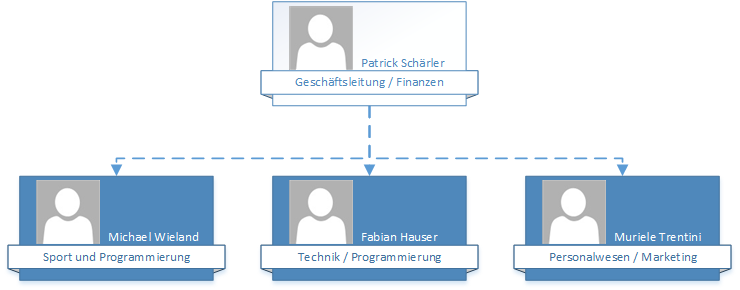
\includegraphics[width=0.9\linewidth]{images/organigramm}
	\caption{Organigramm}
	\label{fig:organigramm}
\end{figure}

\clearpage

\subsection{Das Team}

\subsubsection{Patrick Scherler}
\noindent\begin{minipage}{0.7\textwidth}
	\paragraph{Kontakt} \hfill \\
	Patrick Scherler \\
	Tannenstrasse 4 \\
	9242 Oberuzwil \\
	
	\paragraph{Funktion} \hfill \\
	Partner, Geschäftsleitung, Entwicklung \\
	
	\paragraph{Ausbildung} \hfill \\
	2009-2013 \hspace{1cm} Berufslehre zum Informatiker EFZ \\
	2013-2015 \hspace{1cm} Automation Engineer, Bühler AG \\
	seit 2015 \hspace{1.25cm} Informatik Studium an der HSR \\
		
	\paragraph{Hobbies} \hfill \\
	Kung Fu, Jungschar \\
\end{minipage}
\hfill
\begin{minipage}{0.3\textwidth}\raggedright
	
\includegraphics[width=\textwidth]{images/team/pscherler}
\end{minipage}

\subsubsection{Michael Wieland}
\noindent\begin{minipage}{0.7\textwidth}
	\paragraph{Kontakt} \hfill \\
	Michael Wieland \\
	Löwengasse 1 \\
	7208 Malans \\
	
	\paragraph{Funktion} \hfill \\
	Partner, Sport, Marketing, Entwicklung \\
	
	\paragraph{Ausbildung} \hfill \\
	2008-2012 \hspace{1cm} Berufslehre zum Informatiker EFZ \\
	2012-2014 \hspace{1cm} Software Entwickler \\
	2014-2015 \hspace{1cm} Auslandaufenthalt \\
	seit 2015 \hspace{1.25cm} Informatik Studium an der HSR \\
	
	\paragraph{Hobbies} \hfill \\
	Unihockey, Fussball, Fitness, Bass
\end{minipage}
\hfill
\begin{minipage}{0.3\textwidth}\raggedright
	
\includegraphics[width=\textwidth]{images/team/mwieland}
\end{minipage}

\clearpage


\subsubsection{Murièle Trentini}
\noindent\begin{minipage}{0.7\textwidth}
	\paragraph{Kontakt} \hfill \\
	Murièle Trentini \\
	Rickenstrasse 7 \\
	8634 Hombrechtikon \\
	
	\paragraph{Funktion} \hfill \\
	Partner, Personalwesen, Entwicklung \\
	
	\paragraph{Ausbildung} \hfill \\
	2003-2007 \hspace{1cm} MNG Rämibühl: Matura \\
	2010-2013 \hspace{1cm} Biomedizinische Analytikerin HF \\
	seit 2015\hspace{1.35cm} Informatik Studium an der HSR\\
	
	\paragraph{Hobbies} \hfill \\
	Segeln, Lesen \\
\end{minipage}
\hfill
\begin{minipage}{0.3\textwidth}\raggedright
	
\includegraphics[width=\textwidth]{images/team/mtrentini}
\end{minipage}

\subsubsection{Fabian Hauser}
\noindent\begin{minipage}{0.7\textwidth}
	\paragraph{Kontakt} \hfill \\
	Fabian Hauser \\
	Seewiesstrasse 2 \\
	8640 Rapperswil \\
	
	\paragraph{Funktion} \hfill \\
	Partner, Finanzen, Entwicklung \\
	
	\paragraph{Ausbildung} \hfill \\
	2010-2014 \hspace{1cm} Berufslehre zum Informatiker EFZ \\
	2014-2015 \hspace{1cm} System Engineer, Somedia AG \\
	seit 2015 \hspace{1.25cm} Informatik Studium an der HSR \\
	
	\paragraph{Hobbies} \hfill \\
	Fotografieren, Lesen \\
\end{minipage}
\hfill
\begin{minipage}{0.3\textwidth}\raggedright
	
\includegraphics[width=\textwidth]{images/team/fhauser}
\end{minipage}

\clearpage
\section{Chancen und Risiken: eine ehrliche Bilanz}

Dieses Kapitel listet kritische Ereignisse auf, welche ein Risiko für unser Unternehmen darstellen. Diese Risiken werden nach ihrer Eintrittswahrscheinlichkeit und dem Schadenspotential gewichtet und in einer Matrix analysiert.

\subsection{Risiken}
Nachfolgend sind die wahrscheinlichsten Ereignisse aufgelistet und kurz beschrieben:
\\ \\
\begin{tabu} to \linewidth {l X}
	Wenig Absatz & Unser Produkt stösst auf wenig Begeisterung und wir können nicht genügend Kunden akquirieren. \newline \\
	Keine Grosskunden & Dies ist als separater Punkt aufgeführt, da unsere Strategie das akquirieren von Fitnesscenter-Ketten vorsieht. \newline \\
	Konkurrenz & Das plötzliche Auftauchen eines neuen Mitbewerbers oder die Veränderung einer bestehenden Konkurrenzbeurteilung. \newline \\
	Applikationsausfall & Das Ausfallen unserer Applikation in der Cloud führt zu einem Unterbruch in der Verfügbarkeit unserer App. \newline \\
	Datendiebstahl & Das mutwillige Entwenden von Kundendaten durch eine Drittperson. \newline \\ 
	Datenverlust & Der unwiderrufliche Verlust von gespeicherten Kundendaten. \newline \\
\end{tabu}
\\
\clearpage

\noindent In der Tabelle sind die Ereignisse absteigend nach ihrem geschätzten Schadenspotential aufgeführt. Das Risiko entspricht dem Produkt des Schadenspotentials und der Eintrittswahrscheinlichkeit.
\begin{table}[H]
	\centering
	\begin{tabu} to \linewidth {l l l l}
		\toprule
		Ereignis & Schadenspotential & Eintrittswahrscheinlichkeit & Risiko \\
		\midrule
		Wenig Absatz & 4 & 4 & 16 \\
		Keine Grosskunden & 3 & 3 & 9 \\
		Konkurrenz & 3 & 2 & 6 \\
		Applikationsausfall & 1 & 2 & 2 \\
		Datendiebstahl & 2 & 1 & 2 \\
		Datenverlust & 1 & 1 & 1 \\
		\bottomrule
	\end{tabu}
	\label{tbl:risikoanalyse}
	\caption{Risikoanalyse der wahrscheinlichsten Ereignisse}
\end{table}

\noindent Aus den oben berechneten Daten ergibt sich folgendes Diagramm zur einfacheren Risikobeurteilung. Die Kreise entsprechen den Ereignissen und deren Grösse dem jeweiligen Risiko.
\begin{figure}[H]
	\centering
	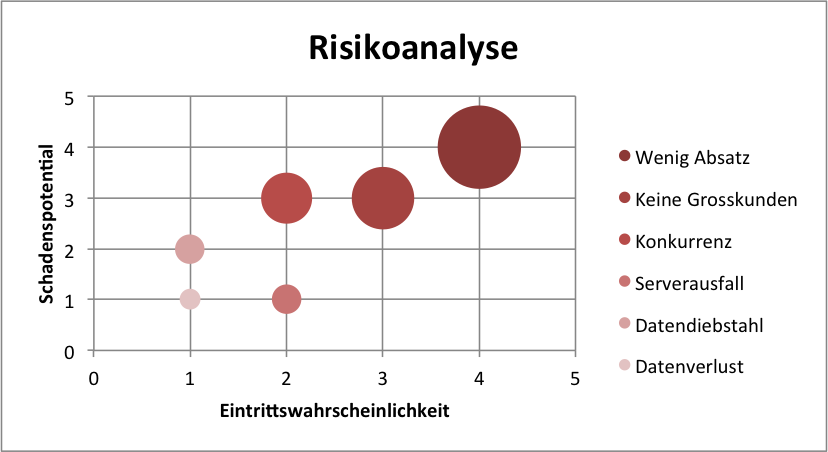
\includegraphics[width=0.8\linewidth]{images/risikoanalyse}
	\caption{Visualisierung der Risikoanalyse}
	\label{fig:visualisierung-risikoanalyse}
\end{figure}

\subsection{Massnahmen}
Zur Reduzierung des Risikos kann entweder das Schadenspotential oder die Eintrittswahrscheinlichkeit verringert werden.
\paragraph{Wenig Absatz}
Das Risiko von zu wenig Absatz ist zwar relativ gross, besteht allerdings vorwiegend zu Beginn der Markteinführung, da unsere Kundenbindung relativ hoch ist. Sobald eine gewisse Menge an Kunden akquiriert ist und daraus Gewinn generiert wird, senkt sich die Eintrittswahrscheinlichkeit beträchtlich. Als Sicherheit sollte hier die Mindestanzahl Kunden berechnet werden, um noch rentabel zu sein. 
\paragraph{Keine Grosskunden}
Das Ausbleiben von Grosskunden wäre ein herber Schlag für unser Unternehmen. Man müsste das Konzept und den Werbeauftritt grundlegend überarbeiten oder die Strategie anpassen und erst auf kleinere Fitnesscenter fokussieren.
\paragraph{Konkurrenz}
Sollte sich die Konkurrenzsituation unerwartet schnell ändern, stellt dies vor allem eine Gefahr dar, solange der Kundenstamm noch relativ klein ist. Eine solide Kundenbasis würde Sicherheit bringen, da die Kundenbindung unseres Produkts eher hoch ist.
\paragraph{Applikationsausfall, Datendiebstahl und –Verlust}
Das Behandeln dieser Probleme kann durch gängige technische Mittel relativ einfach umgesetzt werden. Durch ein ausgeklügeltes Qualitätsmanagement verhindern wir Ausfälle in unserer Applikation.  Verschlüsselung und Sicherheitstechnologien bieten Schutz vor Datendiebstählen.

\subsection{SWOT-Analyse}

Die SWOT-Analyse stellt unsere internen Stärken und Schwächen den externen Chancen und Gefahren gegenüber. Dies dient der Positionsbestimmung und bietet die Grundlage für eine realistische Strategieentwicklung.

\begin{table}[H]
	\centering
	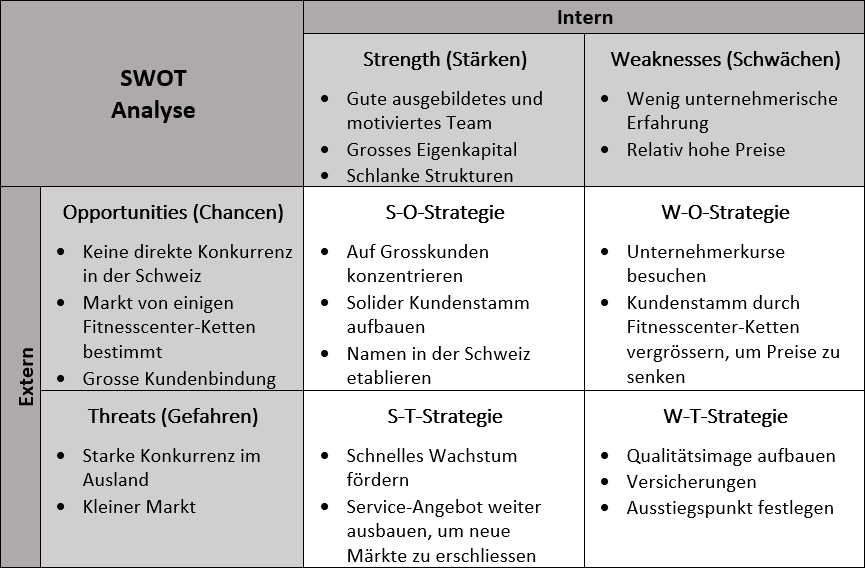
\includegraphics[width=1\linewidth]{images/SWOT-analyse}
	\caption{SWOT Analyse der Chancen und Risiken von GitFit}
	\label{fig:swot-analyse}
\end{table}

\clearpage
\section{Finanzieller Teil: die nackten Zahlen}

Die Finanzpläne sind dem Anhang \ref{appendix:finanzplan} zu entnehmen.

\subsection{Berechnungsgrundlagen}

\subsubsection{Arbeitsplätze}

In den ersten drei Jahren arbeiten alle Mitarbeiter von privaten Arbeitsplätzen zu Hause aus (''Working from Home''). Dies ist dank unserer digitalen Lösung möglich.

\subsubsection{Schulungen und Margen auf verkaufte Geräte}
Die Einnahmen durch Schulungen und Margen auf verkaufte Geräte sind ungefähr linear zu den Einnahmen durch das Abomodell. Wir schätzen diese auf ca. 8\% der Abokosten. 
Dies entspricht ungefähr dem Mehrwertssteuersatz und wird deshalb nicht explizit im Finanzplan aufgeführt.

\subsubsection{Kundenzahlen / Aboumsatz}

Der Tabelle \ref{tbl:kundenzahlen-aboumsatz} können die angestrebten Accountzahlen abgelesen werden. Auf der Basis dieser Werte basieren die im Finanzplan angegebenen Zahlen.

\begin{table}[h]
	\centering
	\begin{tabu} to \linewidth {l l l}
		\toprule
		Jahr & Fitnesscenter & Mitglieder/Center (im $\varnothing$) \\
		\midrule
		2016 & 3 & 500 \\
		2017 & 30 & 450 \\
		2018 & 150 & 400 \\
		\bottomrule
	\end{tabu}
	\label{tbl:kundenzahlen-aboumsatz}
	\caption{Geplante Accountzahlen / Aboumsatz}
\end{table}

\subsubsection{Kosten für das Cloud-Hosting}
Die Kosten für das Cloud-Hosting sind abhängig von der Anzahl verpflichteten Abonnenten; damit skalieren die Kosten gleichmässig mit dem Umsatz und betragen ca. 1\% der eingenommenen Abonnementsgebühren.

\subsubsection{Personalkosten}
In den ersten zwei Jahren rechnen wir mit den 4 Gründungsmitglieder à 6000.- Brutto (aus betrieblicher Sicht, exkl. Steuerabzüge). Im dritten Jahr werden zwei weitere MitarbeiterInnen im Bereich Verkauf zu den selben Konditionen eingestellt.



\clearpage
\section{Umsetzungsplan: die Realisierung}
Musste nicht bearbeitet werden

\clearpage
\appendix

% List of figures
\listoffigures

% List of tables
\listoftables

% Bibliography
\bibliographystyle{plain} 
\bibliography{literatur}

\end{document}
